\documentclass[letterpaper, twoside, 12pt,memoire]{thETS}
\usepackage{amsmath}
\usepackage{amsfonts}
\usepackage{amssymb}
\usepackage[utf8]{inputenc}
\usepackage{graphicx}
\usepackage{color}
\usepackage[T1]{fontenc}
\usepackage{subfigure}
\usepackage{setspace}
\usepackage{todonotes}
\usepackage{varwidth}
\usepackage{float}
\usepackage[section]{placeins}
\usepackage[round]{natbibETS}
\usepackage[mathcal]{euscript}
\usepackage{enumerate}
\usepackage{tikz}
\usepackage{import}

\hyphenpenalty=5000
\tolerance=1000

\newcommand{\ang}[1]{(\textit{#1})}
\newcommand{\bul}{$\quad\bullet$~~}
\newcommand{\fig}[1]{figure~\ref{#1}}
\newcommand{\ltCodec}{logiciel de référence H.264/AVC JM}
\newcommand{\sect}[1]{section~\ref{#1}}

\newcommand{\LT}[1]{%
	{
	\todo[inline,color={red!33!green!33!blue!33}]{%
	\textbf{[LT]:}~#1}
	}}
	
\newcommand{\SC}[1]{%
	{
	\todo[inline,color={red!100!green!33!}]{%
	\textbf{[SC]:}~#1}
	}}

\begin{document}
\begin{chapter}{Le transport de séquences H.264}
Au chapitre précédent, nous avons décrit sommairement la norme de codage H.264.
Dans ce chapitre, il sera question des considérations de transport d'une
séquence H.264 sur des réseaux peu fiables. La norme H.264 inclut plusieurs
mécanismes permettant d'améliorer la résilience aux erreurs et l'empaquetage
d'une séquence vidéo encodée.

Tout d'abord, la notion de tranche, décrite au chapitre précédent, est
revisitée à la \sect{sect-tranche}, mais cette fois, dans l'optique du
transport sur des réseaux peu fiables. Par la suite, à la
\sect{sect-dissimulation}, nous présentons des algorithmes de dissimulation de
paquets perdus. Après quoi, d'autres approches de résilience aux erreurs sont
décrites : l'ordonnancement flexible de macroblocs, à la \sect{sect-FMO}, ainsi que les
ensembles de paramètres, à la \sect{sect-ParameterSets}. Finalement, aux
sections~\ref{sect-NAL} et \ref{sect-RTP}, des notions en lien avec la
réseautique sont présentées, soit la couche d'abstraction réseau et la
hiérarchie protocolaire RTP/UDP/IP.


\begin{section}{Les tranches}
\label{sect-tranche}
Nous avons déjà mentionné, lors de notre description de la norme H.264, la
notion de tranche. On définit une tranche comme un regroupement de macroblocs encodés indépendamment du
contenu des autres macroblocs de la trame. En ce qui a trait à la résilience aux
erreurs, l'usage de tranches offre deux avantages intéressants: empêcher la
propagation d'erreurs et réduire les données manquantes lors de la perte de
paquets. La séparation du contenu de la trame en plusieurs paquets fait en sorte
que si un de ceux-ci est perdu, ce n'est pas la trame entière qui est perdue,
mais seulement le contenu de la tranche manquante. Typiquement, l'assignation
des macroblocs à une tranche se fait par un ordonnancement séquentiel de gauche
à droite et du haut vers le bas \ang{raster}. Comme illustré à la
\fig{fig-Tranches}, où les 99 macroblocs d'une trame QCIF sont regroupés à
l'intérieur de trois tranches.

\begin{figure}[htb] \centering
%% Creator: Inkscape inkscape 0.48pre0, www.inkscape.org
%% PDF/EPS/PS + LaTeX output extension by Johan Engelen, 2010
%% Accompanies image file 'Tranches' (pdf, eps, ps)
%%
%% To include the image in your LaTeX document, write
%%   \input{<filename>.tex}
%%  instead of
%%   \includegraphics{<filename>.pdf}
%% To scale the image, write
%%   \def{\svgwidth}{<desired width>}
%%   \input{<filename>.tex}
%%  instead of
%%   \includegraphics[width=<desired width>]{<filename>.pdf}

\begingroup
  \makeatletter
  \providecommand\color[2][]{%
    \errmessage{(Inkscape) Color is used for the text in Inkscape, but the package 'color.sty' is not loaded}
    \renewcommand\color[2][]{}%
  }
  \providecommand\transparent[1]{%
    \errmessage{(Inkscape) Transparency is used (non-zero) for the text in Inkscape, but the package 'transparent.sty' is not loaded}
    \renewcommand\transparent[1]{}%
  }
  \providecommand\rotatebox[2]{#2}
  \ifx\svgwidth\undefined
    \setlength{\unitlength}{224.4pt}
  \else
    \setlength{\unitlength}{\svgwidth}
  \fi
  \global\let\svgwidth\undefined
  \makeatother
  \begin{picture}(1,0.82070107)%
    \put(0,0){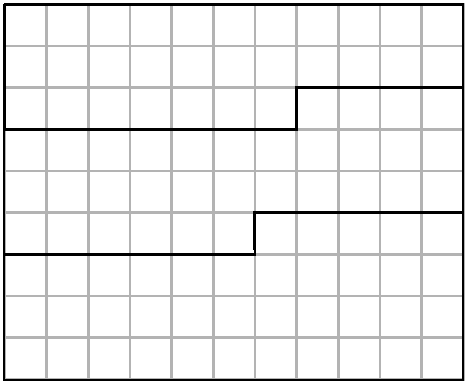
\includegraphics[width=\unitlength]{images/Tranches.pdf}}%
    \put(0.3877749,0.75127634){\color[rgb]{0,0,0}\makebox(0,0)[lb]{\smash{Tranche \#0}}}%
    \put(0.3899317,0.48389664){\color[rgb]{0,0,0}\makebox(0,0)[lb]{\smash{Tranche \#1}}}%
    \put(0.38792113,0.21651699){\color[rgb]{0,0,0}\makebox(0,0)[lb]{\smash{Tranche \#2}}}%
  \end{picture}%
\endgroup

\caption{Séparation des macroblocs d'une trame QCIF en trois tranches.\\Adaptée
de \citet[p.~556]{wiegand2003}}
\label{fig-Tranches}
\end{figure}

Cependant, il y a des désavantages reliés à l'usage des tranches. Premièrement,
les résultats des prédictions sont parfois moins précis, vu qu'elles sont
restreintes à utiliser uniquement le contenu de la tranche. Par exemple, le bloc offrant la meilleure prédiction pourrait être à l'extérieur de la tranche. Deuxièmement, les
tranches augmentent le ratio de données d'entête par rapport aux données vidéo.
Comme présenté à la \sect{sect-RTP}, chaque tranche doit avoir un entête NAL,
ainsi que les entêtes des protocoles RTP, UDP et IP.
\SC{ réduit les délais de quoi puisqu'à la fin il faut les attendre?}
Le regroupement de macroblocs à l'intérieur de tranches permet aussi d'envoyer
ces dernières séparément. De plus, la norme H.264 prévoit la notion
d'ordonnancement arbitraire des tranches \ang{Arbitrary Slice Order (ASO)}.
L'ASO permet la transmission des tranches dans le désordre. Ceci réduit
considérablement les délais sur des réseaux, où il n'y a pas de garantie de
l'ordre de livraison des paquets,



 tels les réseaux IP \citep{sullivan2005}.
\end{section}


\begin{section}{Dissimulation d'erreurs dans le décodeur H.264}
\label{sect-dissimulation}
La perte de paquets est omniprésente sur les réseaux peu fiables. Soit parce que
ceux-ci ne se rendent pas à destination dans les délais requis, ou parce qu'ils
sont endommagés lors du transport. Le décodeur inclus dans le \ltCodec~ offre
deux options de dissimulation de tranches manquantes : le calque de la
trame\footnoteETS{Traduction employée dans cet ouvrage pour l'expression
\textit{slice copy}.}  et le calque des vecteurs de
mouvement\footnoteETS{Traduction employée dans cet ouvrage pour l'expression
\textit{motion copy}.}.\SC{calque de tranche ou de trame?}

Comme son nom l'indique, le calque de la trame remplace une trame corrompue par
la trame qui la précède. S'il y a plus d'une tranche par trame, alors le
remplacement s'effectue au niveau de la tranche manquante. Tandis que les autres
tranches de la trame sont intactes. Cette approche a deux avantages : le premier
est sa facilité d'implémentation, et le deuxième est son efficacité lorsqu'il y a
peu de variation entre les trames. La \fig{fig-FrameCopy} illustre un exemple où
la deuxième tranche d'une trame est corrompue, le décodeur la remplace par la
deuxième tranche de la trame qui la précède.

\begin{figure}[htb] \fbox{\begin{varwidth}{\textwidth}\centering \tikzstyle{na}
= [Baseline=-.5ex] \tikzstyle{every picture}+=[remember picture]
\subfigure[Trame précédente]{

\begin{tikzpicture}
\node (prev){
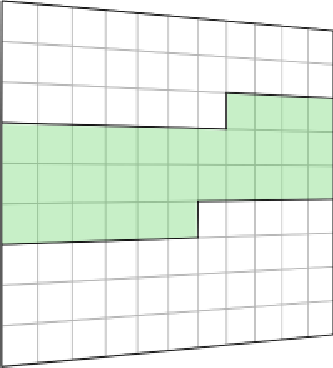
\includegraphics{images/PreviousFrame.pdf}
};
\end{tikzpicture}
\label{fig-PreviousFrame}
} \hspace{3em}
\subfigure[Trame erronée]{
\begin{tikzpicture}
\node (bad) {
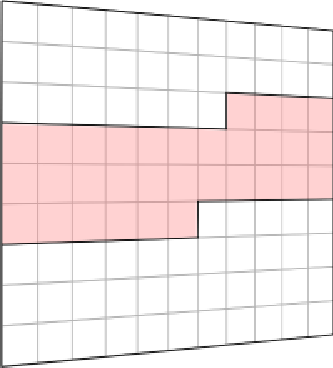
\includegraphics{images/BrokenFrame.pdf}
};
\end{tikzpicture}
\label{fig-BrokenFrame}
}

\begin{tikzpicture}[overlay]
	\path[->, thick] (bad.west) edge [bend right]  (prev.east) ;
\end{tikzpicture}
\end{varwidth}}
\caption{ Visualisation du calque d'une tranche.}
\label{fig-FrameCopy}
\end{figure}

Une autre approche de dissimulation employée par le décodeur inclus dans le
\ltCodec~est le calque des vecteurs de mouvement, comme illustré à la
\fig{fig-MotionCopy}. Cette approche repose sur la corrélation temporelle des
vecteurs de mouvement, proposée par \citet{Wu2006}. Lorsqu'une tranche est
endommagée, les vecteurs de mouvement de la tranche correspondante, dans la
trame précédente, sont réutilisés. Cela a pour effet de perpétuer le
mouvement. Selon \citeauthor{Wu2006}, cette approche est plus efficace que le
calque de la trame lorsqu'il y a du mouvement entre la trame précédente et la
trame erronée.

\begin{figure}[htb]
\fbox{\begin{varwidth}{\textwidth}\centering
\tikzstyle{na} = [Baseline=-.5ex]
\tikzstyle{every picture}+=[remember picture]
\subfigure[Trame précédente]{

\begin{tikzpicture}
\node (prevMV){
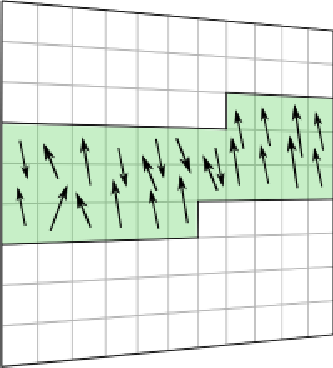
\includegraphics{images/PreviousMVFrame.pdf}
};
\end{tikzpicture}
\label{fig-PreviousFrameMV}
} \hspace{3em}
\subfigure[Trame erronée]{
\begin{tikzpicture}
\node (badMV) {
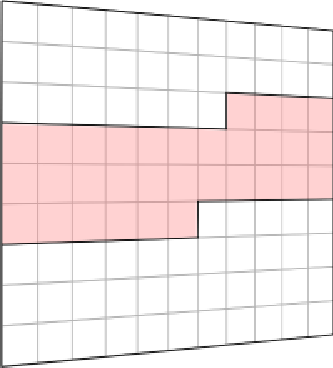
\includegraphics{images/BrokenFrame.pdf}
};
\end{tikzpicture}
\label{fig-BrokenFrame}
}

\begin{tikzpicture}[overlay]
	\path[->, thick] (badMV.west) edge [bend right]  (prevMV.east) ;
\end{tikzpicture}
\end{varwidth}}
\caption{ Visualisation du calque des vecteurs de mouvement.}
\label{fig-MotionCopy}
\end{figure}

\end{section}

\begin{section}{L'ordonnacement flexible de macroblocs}
\label{sect-FMO}
Comme mentionné à la section précédente, seules les tranches endommagées sont
dissimulées. Pour améliorer l'efficacité de l'algorithme de dissimulation, la
norme H.264 prévoit la possibilité de changer l'ordonnancement des macroblocs à
l'intérieur d'une trame. Ce concept se nomme ordonnancement flexible de
macroblocs \ang{Flexible Macroblock Ordering (FMO)}. Cette technique permet un
meilleur contrôle sur la répartition des macroblocs dans les tranches de sorte
à mieux disperser les pertes à travers l'image et ainsi d'augmenter l'efficacité de
la dissimulation.

La \fig{fig-Tranches} montre l'ordonnancement typique d'une séquence H.264. Il
existe plusieurs types d'ordonnancements flexibles. À titre d'exemple, nous
présentons aux figures~\ref{fig-Dispersed} et \ref{fig-Interleaved} les
ordonnancements de macroblocs dispersé et entrelacé. Tous deux illustrent la
répartition des macroblocs d'une trame séparée en deux tranches.

\begin{figure}[htb]
\fbox{\begin{varwidth}{\textwidth}\centering
\subfigure[Ordonnancement dispersé]{
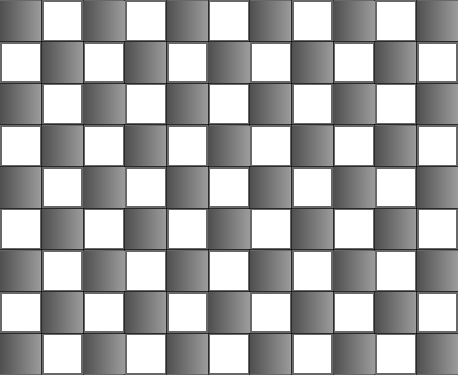
\includegraphics[width=0.47\linewidth]{images/Dispersed.pdf}
\label{fig-Dispersed}
}
\subfigure[Ordonnancement entrelacé]{
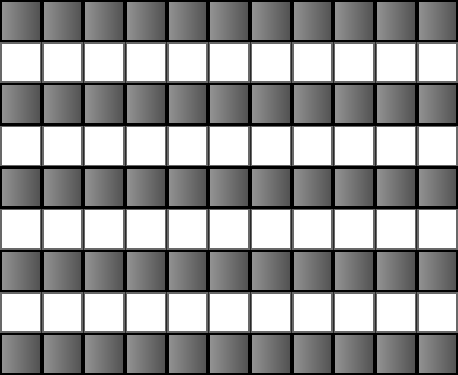
\includegraphics[width=0.47\linewidth]{images/Interleaved.pdf}
\label{fig-Interleaved}
}\\
\subfigure{
\small
\import{images/}{FMOLegend.pdf_tex}
\label{fig-BrokenFrame}
}
\end{varwidth}}
\caption{Exemples d'ordonnancements flexibles de macroblocs pour des trames
QCIF séparées en deux tranches.}
\label{fig-FrameCopy}
\end{figure}

L'ordonnancement dispersé (\ref{fig-Dispersed}) ressemble à un damier, où les
cases alternent d'une tranche à une autre. Ceci fait en sorte que les quatre
voisins d'un macrobloc sont des macroblocs provenant d'autres tranches. Un
exemple de la détérioration visuelle issue du décodage d'une tranche corrompue
contenue dans une trame avec un ordonnancement de type dispersé est présenté à
la \fig{fig-ExempleDisperse}. 

\begin{figure}[htb]
\fbox{\begin{varwidth}{\textwidth}\centering
\subfigure[Trame erronée]{

\includegraphics[width=0.46\linewidth]{images/badCarphoneDispersed.png}
\label{fig-ExempleDisperseErr}
}
\subfigure[Détérioration visuelle (amplifiée)]{
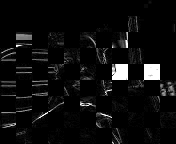
\includegraphics[width=0.46\linewidth]{images/diffCarphoneDispersed.png}
\label{fig-ExempleDisperseDiff}
}
\end{varwidth}}
\caption{Exemple de la détérioration visuelle issue du décodage d'une tranche
corrompue contenue dans une trame avec un ordonnancement de type dispersé.}
\label{fig-ExempleDisperse}
\end{figure}

Pour sa part, l'ordonnancement entrelacé (\ref{fig-Interleaved}) regroupe les
macroblocs en rangées. Celles-ci sont séquentiellement assignées aux tranches de
la trame. Lorsqu'utilisé avec le calquage de tranche, cet ordonnancement permet
de conserver la corrélation spatiale horizontale des macroblocs, au détriment de
la corrélation spatiale verticale. Dans le contexte de notre exemple, une telle
approche de dissimulation fait en sorte que la moitié des rangées de
macroblocs de la trame proviennent de la trame précédente. Un exemple de la
détérioration visuelle issue du décodage d'une tranche corrompue contenue dans
une trame avec un ordonnancement de type entrelacé est présenté à la
\fig{fig-ExempleEntrelace}.

\begin{figure}[htb]
\fbox{\begin{varwidth}{\textwidth}\centering
\subfigure[Trame erronée]{

\includegraphics[width=0.46\linewidth]{images/badCarphoneInterleaved.png}
\label{fig-ExempleEntrelaceErr}
}
\subfigure[Détérioration visuelle (amplifiée)]{
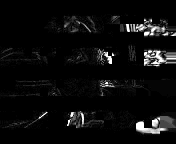
\includegraphics[width=0.46\linewidth]{images/diffCarphoneInterleaved.png}
\label{fig-ExempleEntrelaceDiff}
}
\end{varwidth}}
\caption{Exemple de la détérioration visuelle issue du décodage d'une tranche
corrompue contenue dans une trame avec un ordonnancement de type entrelacé.}
\label{fig-ExempleEntrelace}
\end{figure}

\end{section}

\begin{section}{Les ensembles de paramètres}
\label{sect-ParameterSets}
La notion d'ensembles de paramètres \ang{Parameter sets} augmente
considérablement la résilience aux erreurs, lors du transport d'une séquence
H.264. Ces améliorations sont obtenues par la séparation des paramètres
d'encodage du contenu encodé. En ce qui concerne les normes antérieures, les
paramètres de codages sont souvent inclus dans les mêmes paquets que le contenu
encodé, ce qui augmente la taille des paquets, les rendant ainsi plus susceptibles
d'être erronés. De plus, l'information répétée dans chaque paquet en augmente
considérablement les risques de corruption. Grâce à cette séparation, il est
possible de transmettre ces paramètres de façon plus fiable, afin de s'assurer
leur réception sans erreur. Ils peuvent être aussi transmis plus tôt, afin de
compenser les délais de transport. La norme H.264 prévoit deux types d'ensembles
de paramètres : les paramètres de séquences et les paramètres d'images. Ceux-ci
sont présentés à la \fig{fig-ParameterSet}.

\begin{figure}[htb]
\centering
\fbox{
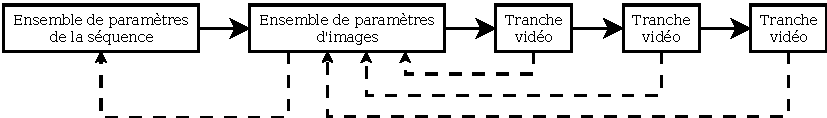
\includegraphics{images/ParameterSet.pdf}
}
\caption{Liens entre les tranches, les ensembles de paramètres d'images et ceux
de la séquence. Adaptée de \citet[p.~53]{Superiori2006}}
\label{fig-ParameterSet}
\end{figure}

Premièrement, il y a les ensembles de paramètres de la séquence. Ceux-ci sont
des paramètres généraux qui régissent la séquence dans son ensemble. Parmi les
paramètres de la séquence, on retrouve: la largeur et la hauteur, en pixels, de la séquence
ainsi que le nombre de trames de référence requises pour le décodage.

Deuxièmement, il y a les ensembles de paramètres d'image qui régissent une ou
plusieurs trames de la séquence. Parmi les paramètres d'image, on retrouve: un
identificateur des paramètres de séquences associés à ces paramètres d'images,
un identifiant permettant d'identifier l'encodage entropique utilisé et le
paramètre de quantification.


\end{section}

\begin{section}{La couche d'abstraction réseau}
\label{sect-NAL}
La norme H.264 sépare les notions de codage vidéo de celles du transport en deux
couches distinctes, comme illustré à la \fig{fig-NAL_VLC}. La couche de codage
vidéo \ang{Video Coding Layer (VCL)} est conçue pour être indépendante du canal
de transmission. Cette couche est présentée en détail dans notre chapitre sur
H.264. La couche d'abstraction réseau \ang{Network Abstraction Layer (NAL)} a
pour responsabilité d'adapter le contenu de la VCL selon les caractéristiques du
canal de transmission afin d'être empaquetée dans des unités NAL. Grâce à cette
couche, la norme H.264 peut être adaptée au transport sur les réseaux de type :
RTP/UDP/IP, H.324M, MPEG-2 TS et H.320 \citep{Wenger2003}.

\begin{figure}[htb]
\centering
\fbox{
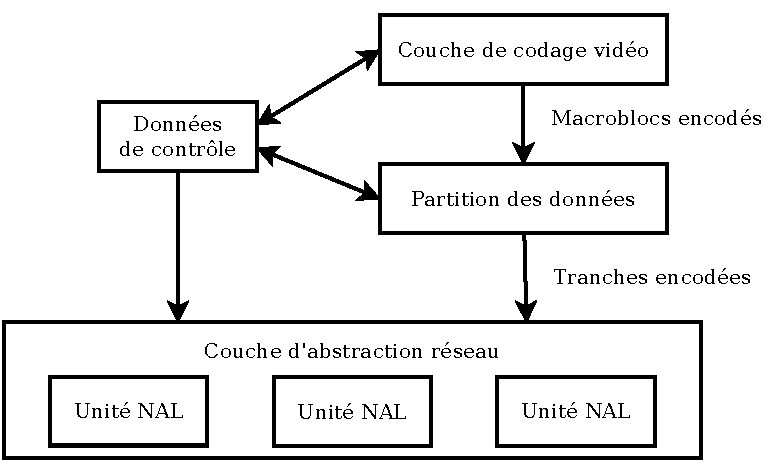
\includegraphics{images/NAL_VLC.pdf}
}
\caption{Liens entre les tranches, les ensemble de paramètre d'image et
de la séquence.\\Adaptée de \citet[p.~53]{Superiori2006}}\SC{Je ne vois pas les paramètres d'image et de séquence dans la figure}
\label{fig-NAL_VLC}
\end{figure}

Une unité NAL \ang{NAL unit} est le nom donné à paquet logique dont le but est
de contenir le contenu provenant de la VCL. Une unité NAL combine un entête NAL
et une séquence d'octets utiles \ang{Raw Byte Sequence Payload (RBSP)}. Ces
octets sont ceux issus de l'encodage d'une séquence H.264.

\LT{Faire le lien avec le chapitre sur H.264}
\end{section}

\begin{section}{La hiérarchie protocolaire RTP/UDP/IP}
\label{sect-RTP}

La hiérarchie protocolaire majoritairement utilisée pour la consultation de flux
vidéo \ang{streaming} et la vidéophonie est RTP/UDP/IP \citep{Wenger2003}. De
par son nom, elle identifie les protocoles utilisés aux couches trois, quatre et
cinq des sept couches du modèle OSI \citep{Zimmermann1980}, comme illustrées à
la \fig{fig-OSI_Layers}. De plus, à la \fig{fig-IPUDPRTP}, nous présentons
l'encapsulation d'une unité NAL pour la hiérarchie protocolaire RTP/UDP/IP. Le
nombre d'octets requis par chaque entête y est aussi indiqué. Ceci nous indique
le fardeau binaire lié à l'encapsulation, soit 40 octets.

\begin{figure}[htb] \centering \fbox{
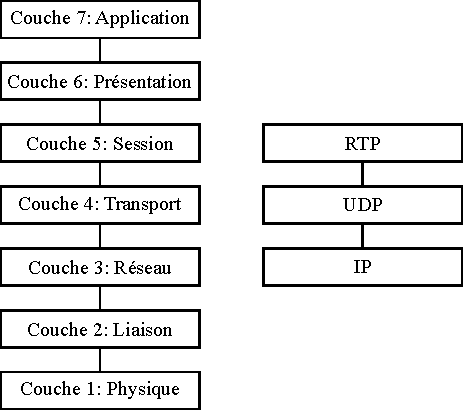
\includegraphics{images/OSI_Layers.pdf}
} \caption{Hiérarchie protocolaire RTP/UDP/IP et les couches du modèle OSI
\\Adaptée de \citet[p.~339]{Smith2006}}
\label{fig-OSI_Layers}
\end{figure}

\begin{figure}[htb] \centering \fbox{
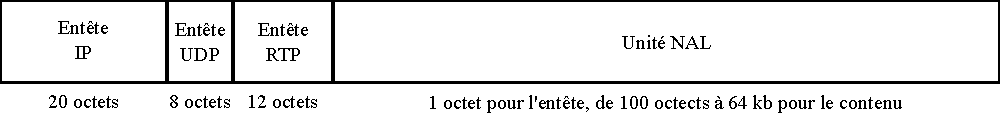
\includegraphics{images/IPUDPRTP.pdf}
} \caption{Données d'entêtes des protocoles IP, UDP, RTP pour l'encapsulation
d'une unité NAL.}
\label{fig-IPUDPRTP}
\end{figure}

Le plus grand avantage d'utiliser le protocole Internet \ang{Internet Protocol
(IP)} est son omniprésence dans le domaine des télécommunications
\citep{Smith2006}. Ce protocole est supporté, non seulement par l'ensemble des
ordinateurs modernes, mais aussi par une panoplie d'appareils portables, tels
les tablettes, les téléphones intelligents ainsi que les décodeurs numériques.
Proprement dit, le protocole IP permet d'acheminer des paquets d'un routeur à
une autre, à travers le réseau, en direction de la destination appropriée
définie par l'adresse de destination IP contenue dans l'entête IP. Cependant, le
protocole IP ne fournit aucune protection contre la perte ou la corruption de
paquets. Notons aussi que le protocole IP ne fournit pas d'information sur
l'ordre de reconstruction des paquets. Pour ce faire, il faudra avoir recours à
des protocoles des couches supérieures.

Le protocole de \textit{datagramme} utilisateur \ang{User Datagram Protocol
(UDP)} réside à la couche quatre du modèle OSI. Il régit un service, simple, de
transport de \textit{datagrammes} sans pour autant en garantir la bonne
livraison. Contrairement à d'autres protocoles de la couche transport, on note
l'absence d'un mécanisme permettant, la validation des \textit{datagrammes}
reçus par le destinataire et leur retransmission au besoin. Ce mécanisme n'étant
pas souhaitable dans nos conditions de transport, car il ajouterait un fardeau
additionnel sur le réseau et dans certains cas, ne permettrait pas de
respecter la contrainte temps réel \citep{Wenger2003}. Toutefois, une somme de
contrôle \ang{checksum} est incluse dans l'entête UDP. Elle permet de valider la
fidélité du \textit{datagramme} reçu. Cependant, notons toujours l'absence
d'information sur l'ordre de reconstruction des paquets.

Au dessus d'UDP, on retrouve le protocole de transmission en temps réel \ang{
real-time transport protocol (RTP)}. Il établit et maintient une session entre
un émetteur et un ou plusieurs destinataires. L'entête de ce protocole est
composé d'informations tels le numéro de séquence, l'estampille temporelle et le
type de données utilisées. Ces informations viennent boucler la boucle en ce qui
concerne le transport de vidéo sur des réseaux peu fiables. Le numéro de
séquence, incrémenté d'un pour chaque paquet de la session, permet d'identifier
les paquets perdus. L'estampille temporelle permet la synchronisation entre
l'émetteur et le destinataire. Les informations sur le type de données utilisées
permettent l'identification de la norme de codage des données, tel H.264.
\end{section}

Ce chapitre sur le transport de séquence H.264, regroupe un grand nombre de
concepts appartenant, d'une part, à la norme de codage H.264, tels les tranches,
la dissimulation d'erreurs, l'ordonnancement flexible de macroblocs, les
ensembles de paramètres et la couche d'abstraction réseau. D'autre part, on
constate des notions de réseautique tels les protocoles IP, UDP et RTP. Même
lorsque tous ces concepts sont employés, il est fort probable que du contenu
vidéo transmis sur un canal de communication peu fiable soit endommagé. Au
prochain chapitre, nous étudions cette erreur, et les conséquences de son
décodage, soit de la détérioration visuelle voire même le plantage du décodeur.

\end{chapter}

\bibliographystyle{bibETS}
\bibliography{h264Transport}

\end{document}
